% Capture overhead per event, by path (E1a/E1b; see tab:overhead for the
% resource and size rows). \input this inside a figure environment;
% needs \usepackage{pgfplots}.
%
% Data: scripts/eval/out/e1a_spool_latency_compute.csv (spool),
%       e1b_emit_collector.csv (collector), e1b_emit_fallback.csv (fallback);
% p50/p95 recomputed from those files and cross-checked against results.md.
%
% NOTE: the category names are used directly as the symbolic y coordinates.
% Do NOT reintroduce a separate `yticklabels={...}` list: with `ytick=data`
% pgfplots orders ticks by their order of appearance in the coordinate list,
% not by the `symbolic y coords` declaration, so a separate label list
% silently attaches the wrong name to each bar.
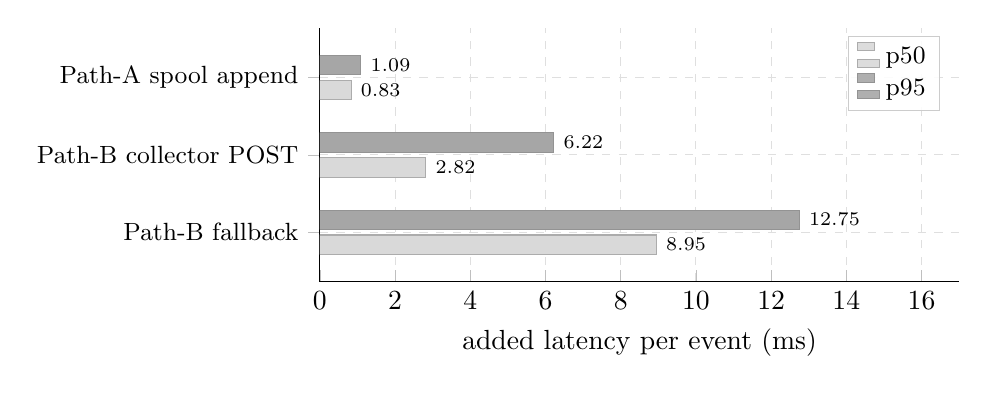
\begin{tikzpicture}
\begin{axis}[
    width=0.80\linewidth, height=4.8cm,
    xbar, bar width=7pt,
    xlabel={added latency per event (ms)},
    xmin=0, xmax=17,
    symbolic y coords={{Path-B fallback},{Path-B collector POST},{Path-A spool append}},
    ytick=data,
    yticklabel style={font=\small},
    nodes near coords, nodes near coords align={horizontal},
    every node near coord/.append style={font=\scriptsize, text=black},
    legend pos=north east, legend cell align=left,
    legend style={font=\small, draw=gray!40, fill=white, fill opacity=0.9,
                  text opacity=1},
    grid=major, grid style={dashed,gray!25},
    enlarge y limits=0.32,
    axis lines*=left,
    tick style={draw=gray!50},
]
\addplot[fill=gray!30, draw=gray!65, mark=none] coordinates {
    (0.83,{Path-A spool append})
    (2.82,{Path-B collector POST})
    (8.95,{Path-B fallback})};
\addplot[fill=gray!70, draw=gray!85, mark=none] coordinates {
    (1.09,{Path-A spool append})
    (6.22,{Path-B collector POST})
    (12.75,{Path-B fallback})};
\legend{p50, p95}
\end{axis}
\end{tikzpicture}
